\documentclass[oneside,a4paper,11pt,explicit]{book}
\usepackage[utf8]{inputenc}
\usepackage{icecream}
\usepackage[english]{babel}
\addto\captionsenglish{\renewcommand{\chaptername}{}}
\usepackage[accsupp]{axessibility}  % improves PDF readability for those with disabilities.
\usepackage[colorlinks = true,urlcolor  = blue,linkcolor = blue]{hyperref}
\usepackage{setspace}
\usepackage{listings}
\usepackage[most]{tcolorbox}
\usepackage{minitoc}


\renewcommand{\mtifont}{\large\sffamily}
\renewcommand{\mtcfont}{\small\sffamily}
\renewcommand{\mtcSfont}{\small\sffamily}
\renewcommand{\mtcSSfont}{\small\sffamily}
\renewcommand{\mtcSSSfont}{\small\sffamily}
\mtcsetpagenumbers{minitoc}{off} % turn off page numbering in minitocs
\addto{\captionsenglish}{% Making babel aware of special titles
	\renewcommand{\mtctitle}{Quick Links To Sections}
}
\setlength{\fboxrule}{5pt}
\setlength{\fboxsep}{4pt}

\definecolor{IceCreamLeaf}{rgb}{0.4, 0.639215686274, 0.4}
\definecolor{IceCreamOrbit}{rgb}{0.803921568627451, 0.3607843137254902, 0.3607843137254902}

\pretolerance=10000
\tolerance=2000 
\emergencystretch=10pt

%%%%%%%%%%%%%%% END PREAMBLE

\title{I.C.E.C.R.E.A.M. Tutorials}
\subtitle{\small Observing Earth from Above (Env 329) v24.06  \\
	\small Schmid College of Science and Technology, Chapman University}
\date{\today}

%% DOCUMENT
\setstretch{1.25}
\makeatletter
\begin{document}
	
\dominitoc
	
\faketableofcontents
	
\setcounter{chapter}{2} %Insert (Tutorial Number-1) Here; example for tutorial 4, enter 3
	
\chapter{Drawing An Area of Interest} %Enter Tutorial Name Here
	
\vspace{-2em}
	
\minitoc
	
\hrule
	
\vspace{1em}
	
\begin{tcolorbox}[enhanced,frame style image=blueshade.png, opacityback=0.75,opacitybacktitle=0.25,colback=blue!5!white,colframe=blue!75!black,title={\Large \textbf{Objectives:}}]
	\large
	\begin{enumerate}
		\item Learn to about the common file types we use everyday in Geographic Information Systems.
		\item Create a shapefile for your hometown or favorite place you have lived in QGIS. 
	\end{enumerate}
\end{tcolorbox}
	
\clearpage
	
%%%%%%%%%%%%%%%%%%%%%%%%%%%%%%%%%% Change Header to Have a Smaller Logo for Remainder of the Document
\fancyhead{}
\fancyhead[C]{\begin{tikzpicture}[overlay, remember picture]
		\fill[Blue2] (current page.north west) rectangle ($(current page.north east)+(0,-1in)$);
		\node[anchor=north west, text=white, font=\Large, minimum size=1in, inner xsep=5mm, align=left] at (current page.north west) {\bf{\MakeUppercase{\@title}}\\\@subtitle};
		\node[anchor=north east, minimum size=1in, inner xsep=5mm] at (current page.north east) {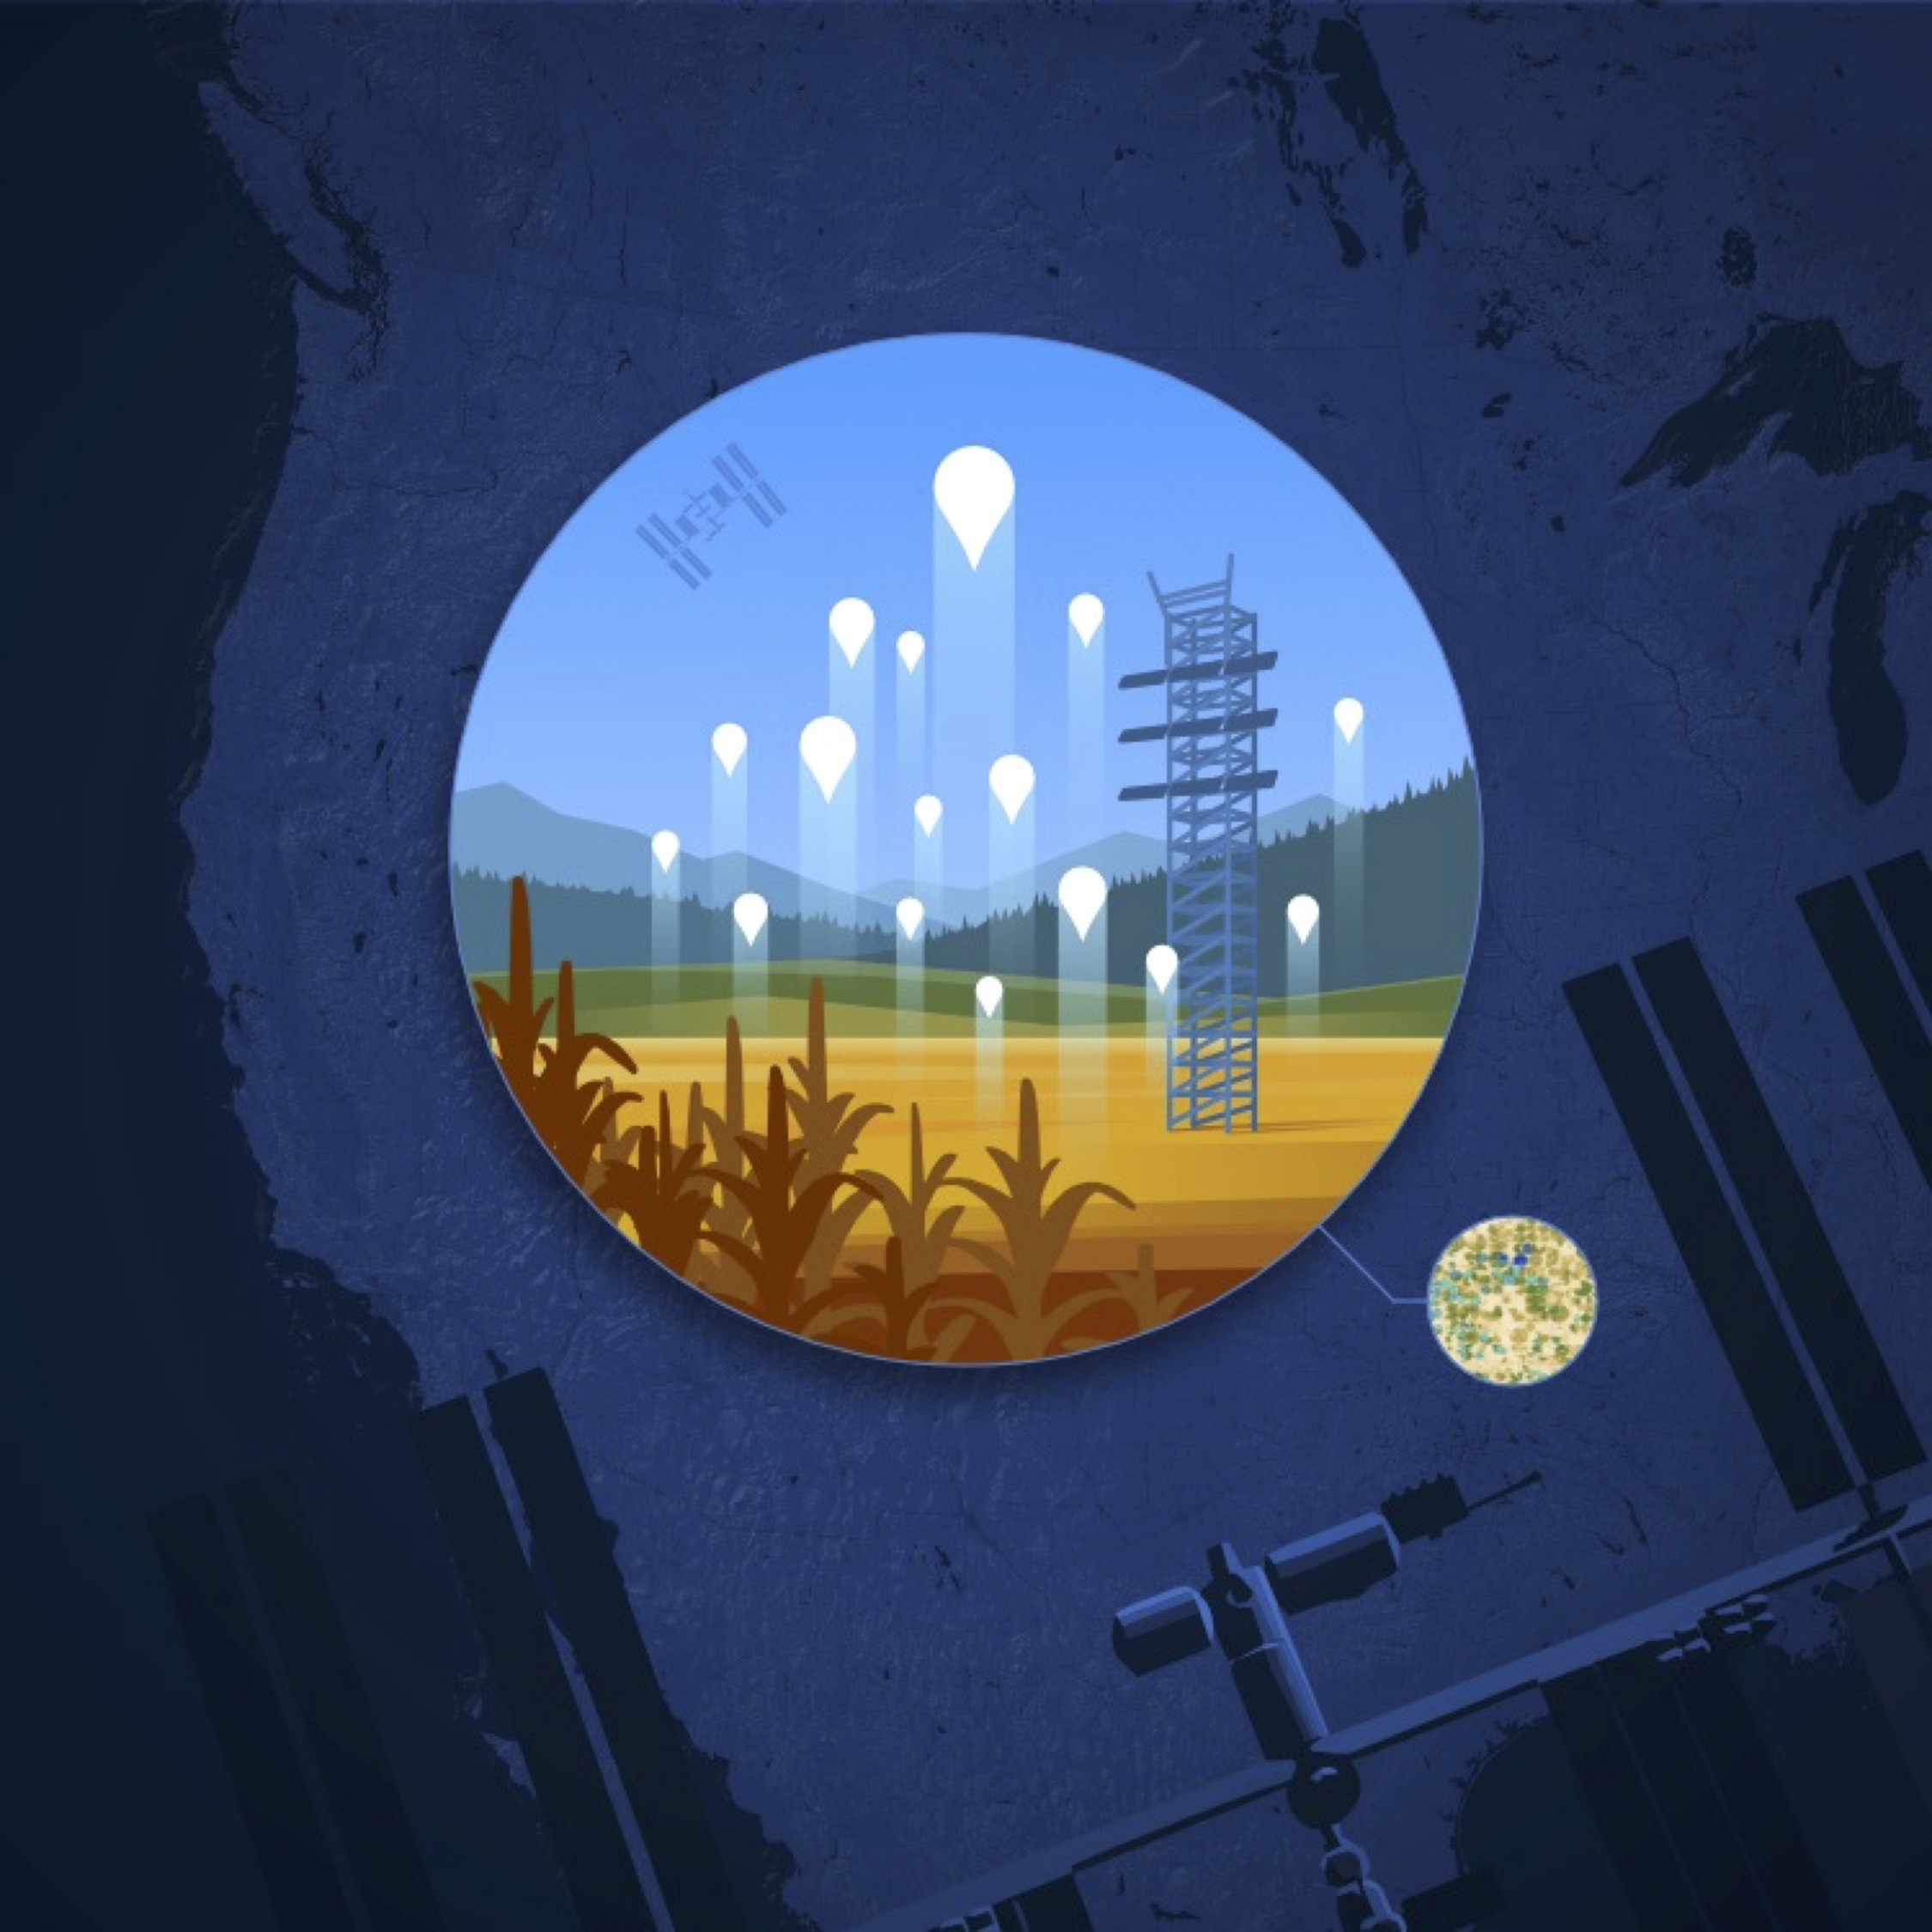
\includegraphics[scale=.03]{ECOSTRESS-BASE.jpg}};\end{tikzpicture}}
%%%%%%%%%%%%%%%%%%%%%%%%%%%%%%%%%%
	
	\noindent\fbox{\begin{minipage}{.9665\textwidth}
			
			\vspace{1em}
			\begin{center}
				\textbf{\Large \underline{Motivation For Today's Tutorial: Temperature Competition}}
			\end{center}
			
			\vspace{1 em}
			
			\centerline{
\includegraphics[width=.75\textwidth]{Hometown.png}}
			
			\vspace{1 em}
			
			
			In the next few tutorials, our goal is to increase the tools you have in your toolkit. In the process, we are going to figure out who has the hottest and coldest temperatures in their hometown or favorite place they have lived. To get started, we need to learn about one of the main tools we use everyday in GIS: vector files. 
			
	\end{minipage}}
	
	\vspace{1 em}

	\section{Area of Interest Data Types For A$\rho\rho$EEARS}

To download ECOSTRESS satellite data, you will need to tell the A$\rho\rho$EEARS data portal what your area of interest (AOI) is. Today, you will learn about the data formats that A$\rho\rho$EEARS accepts as AOI inputs and draw your own AOI polygon. As you can see in the screenshot of the A$\rho\rho$EEARS data portal below, it needs a \textit{vector polygon} to know where to pull ECOSTRESS satellite data for. Before we go any further, we need to discuss the differences between two data types we use daily in geographic information systems (GIS) work, vector and raster data.

\vspace{1em}

\centerline{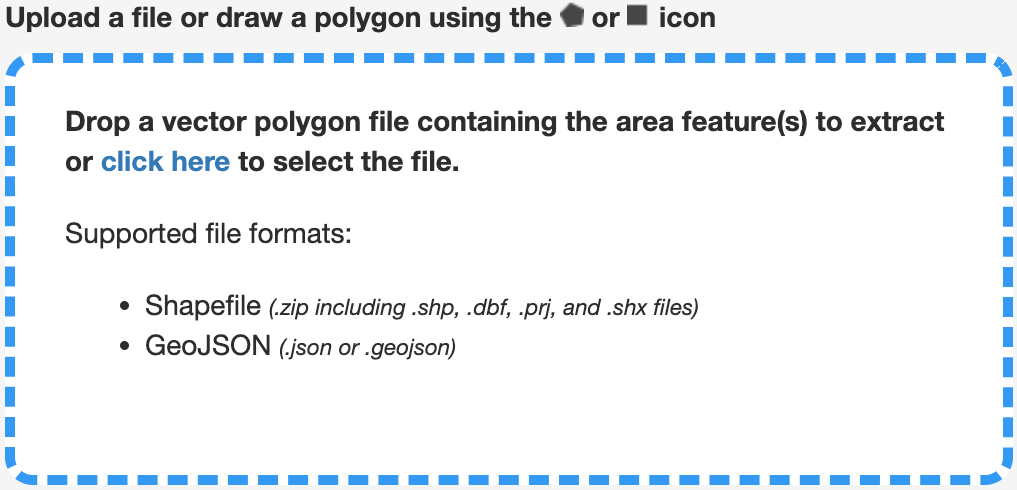
\includegraphics[width=.5\textwidth]{BlankExtract.png}}

\begin{tcolorbox}[colback=yellow!5!white,colframe=IceCreamLeaf,title=\textbf{Vector vs. Raster Data}]

	\centerline{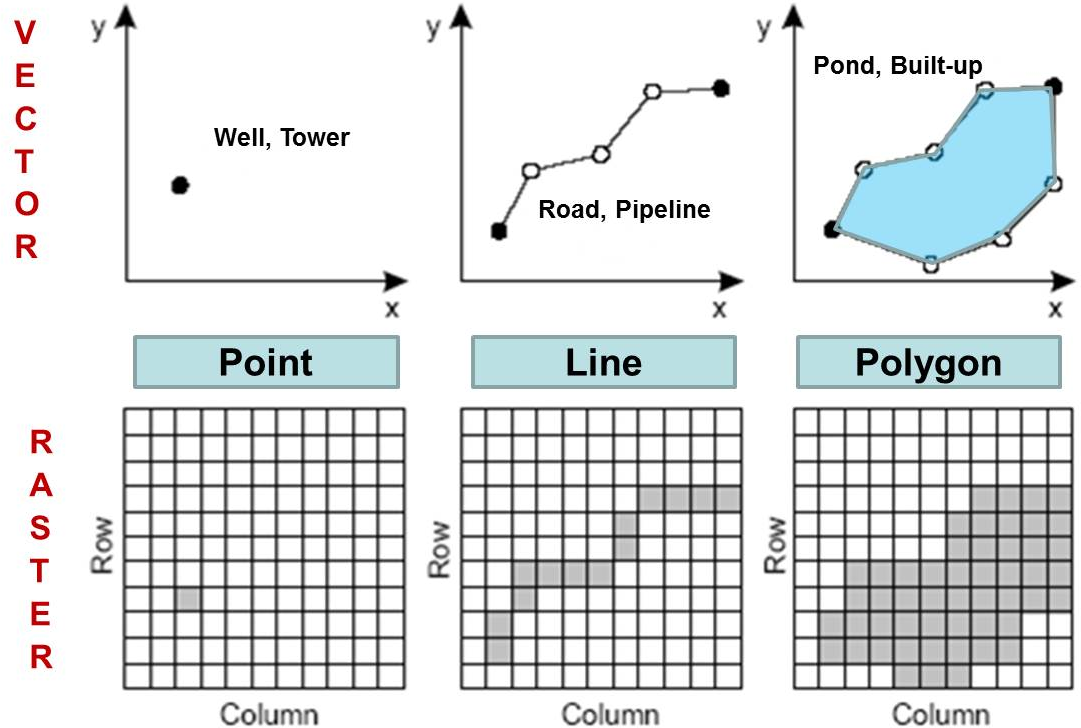
\includegraphics[width=.75\textwidth]{Vector_vs_Raster.png}}

	Both vector and raster data provide different ways to represent real world features within the GIS environment. A feature is anything you can see on the landscape: houses, roads, trees, rivers, etc. 

	\vspace{.5em}

	\textbf{Vector Data:} (Common file formats: Shapefile, GeoJSON, Geopackage)
	\begin{itemize}
		\item A vector feature has its shape represented using geometry. The geometry is made up of one or more interconnected vertices. A vertex describes a position in space using an X, Y, and optional Z axis.
		\item When a feature's geometry consists of only a single vertex, it is referred to as a \textbf{point} feature.
		\item Where the geometry consists of two or more vertices and the first and last vertex are not equal, a \textbf{line} feature is formed.
		\item Where three or more vertices are present, and the last vertex is equal to the first, an enclosed \textbf{polygon} feature is formed. 
		\item Vector features have attributes, which are additional text or numerical data linked to the features that describe something of interest, perhaps a quantitative measure of the severity of a wildfire.
	\end{itemize}

	\vspace{.5em}

	\textbf{Raster Data:} (Common file format: GeoTIFF)
	\begin{itemize}
		\item While vector features use geometry (points, polylines and polygons) to represent the real world, raster data takes a different approach. 
		\item Rasters are made up of a matrix of cells (also called \textbf{pixels}), with each cell containing a value that represents the conditions for the area encompassed by that cell.
		\item Every raster has cells of a fixed size that determine its spatial resolution.
	\end{itemize}
\end{tcolorbox}

A raster approach is best for situations where your data are continuous and vary across space, such as the greenness of grasses in a prairie field or population density in Los Angeles County. The vector approach is better for features that can be represented by points, lines, or polygons, such as trees, hiking trails, or school district boundaries.

\kulbox{\textbf{NOTE:} You can convert between raster and vector file types, but you should have a good reason. For example, if you had vector polygons of wildfires by year and wanted to make a continuous map of burn frequency, you could convert the vectors to rasters to easily add them together. We will revisit raster calculations in a later tutorial.}
	
\section{Creating a Shapefile in QGIS}
	
	Today, you will learn how to create your own polygon vector file in QGIS, but first we are going to make our lives a little easier and expand QGIS's functionality by using a plugin: Lat Lon Tools. \href{https://docs.qgis.org/3.34/en/docs/training_manual/qgis_plugins/fetching_plugins.html}{Plugins} are external pieces of software that add useful features to QGIS. Lat Lon Tools is a plugin that allows us to easily pinpoint a place in QGIS by using its latitude and longitude. 
	
	\subsection{Installing the \textit{Lat Lon Tools} Plugin}
	
	1. Open QGIS and start a new project by selecting the \textit{Project} menu $\rightarrow$ then \textit{New}. 
	
	2. To install the Lat Lon Tools plugin, click on the \textit{Plugins} drop down menu and select \textit{Manage and Install Plugins}.
	
	3. In the next window, make sure \textit{All} is selected in the first window pane and search for \textit{Lat Lon Tools}.
	
	4. Click \textit{Install Plugin}, wait for the installation to complete, then close the plugin window.
	
	\centerline{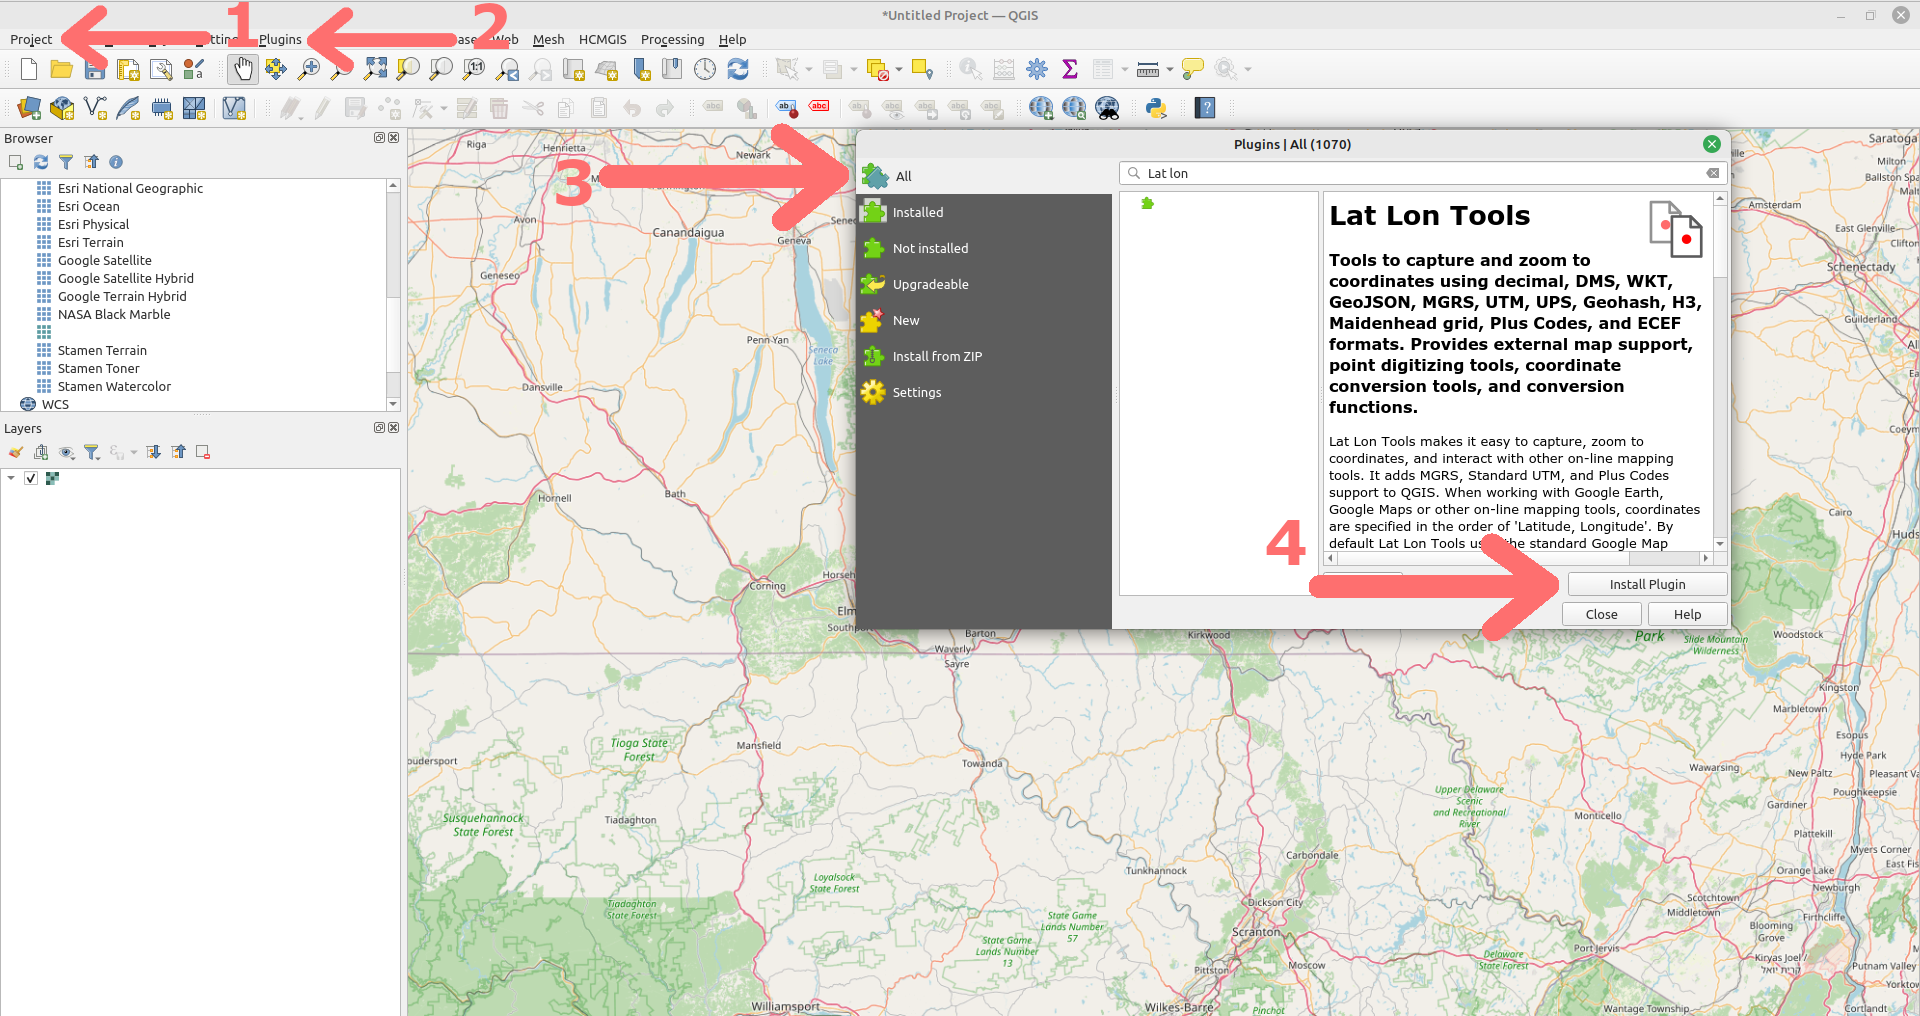
\includegraphics[width=\textwidth]{LatLonTools.png}}
	
	\subsection{Adding an Open Street Basemap Layer}
	
	\centerline{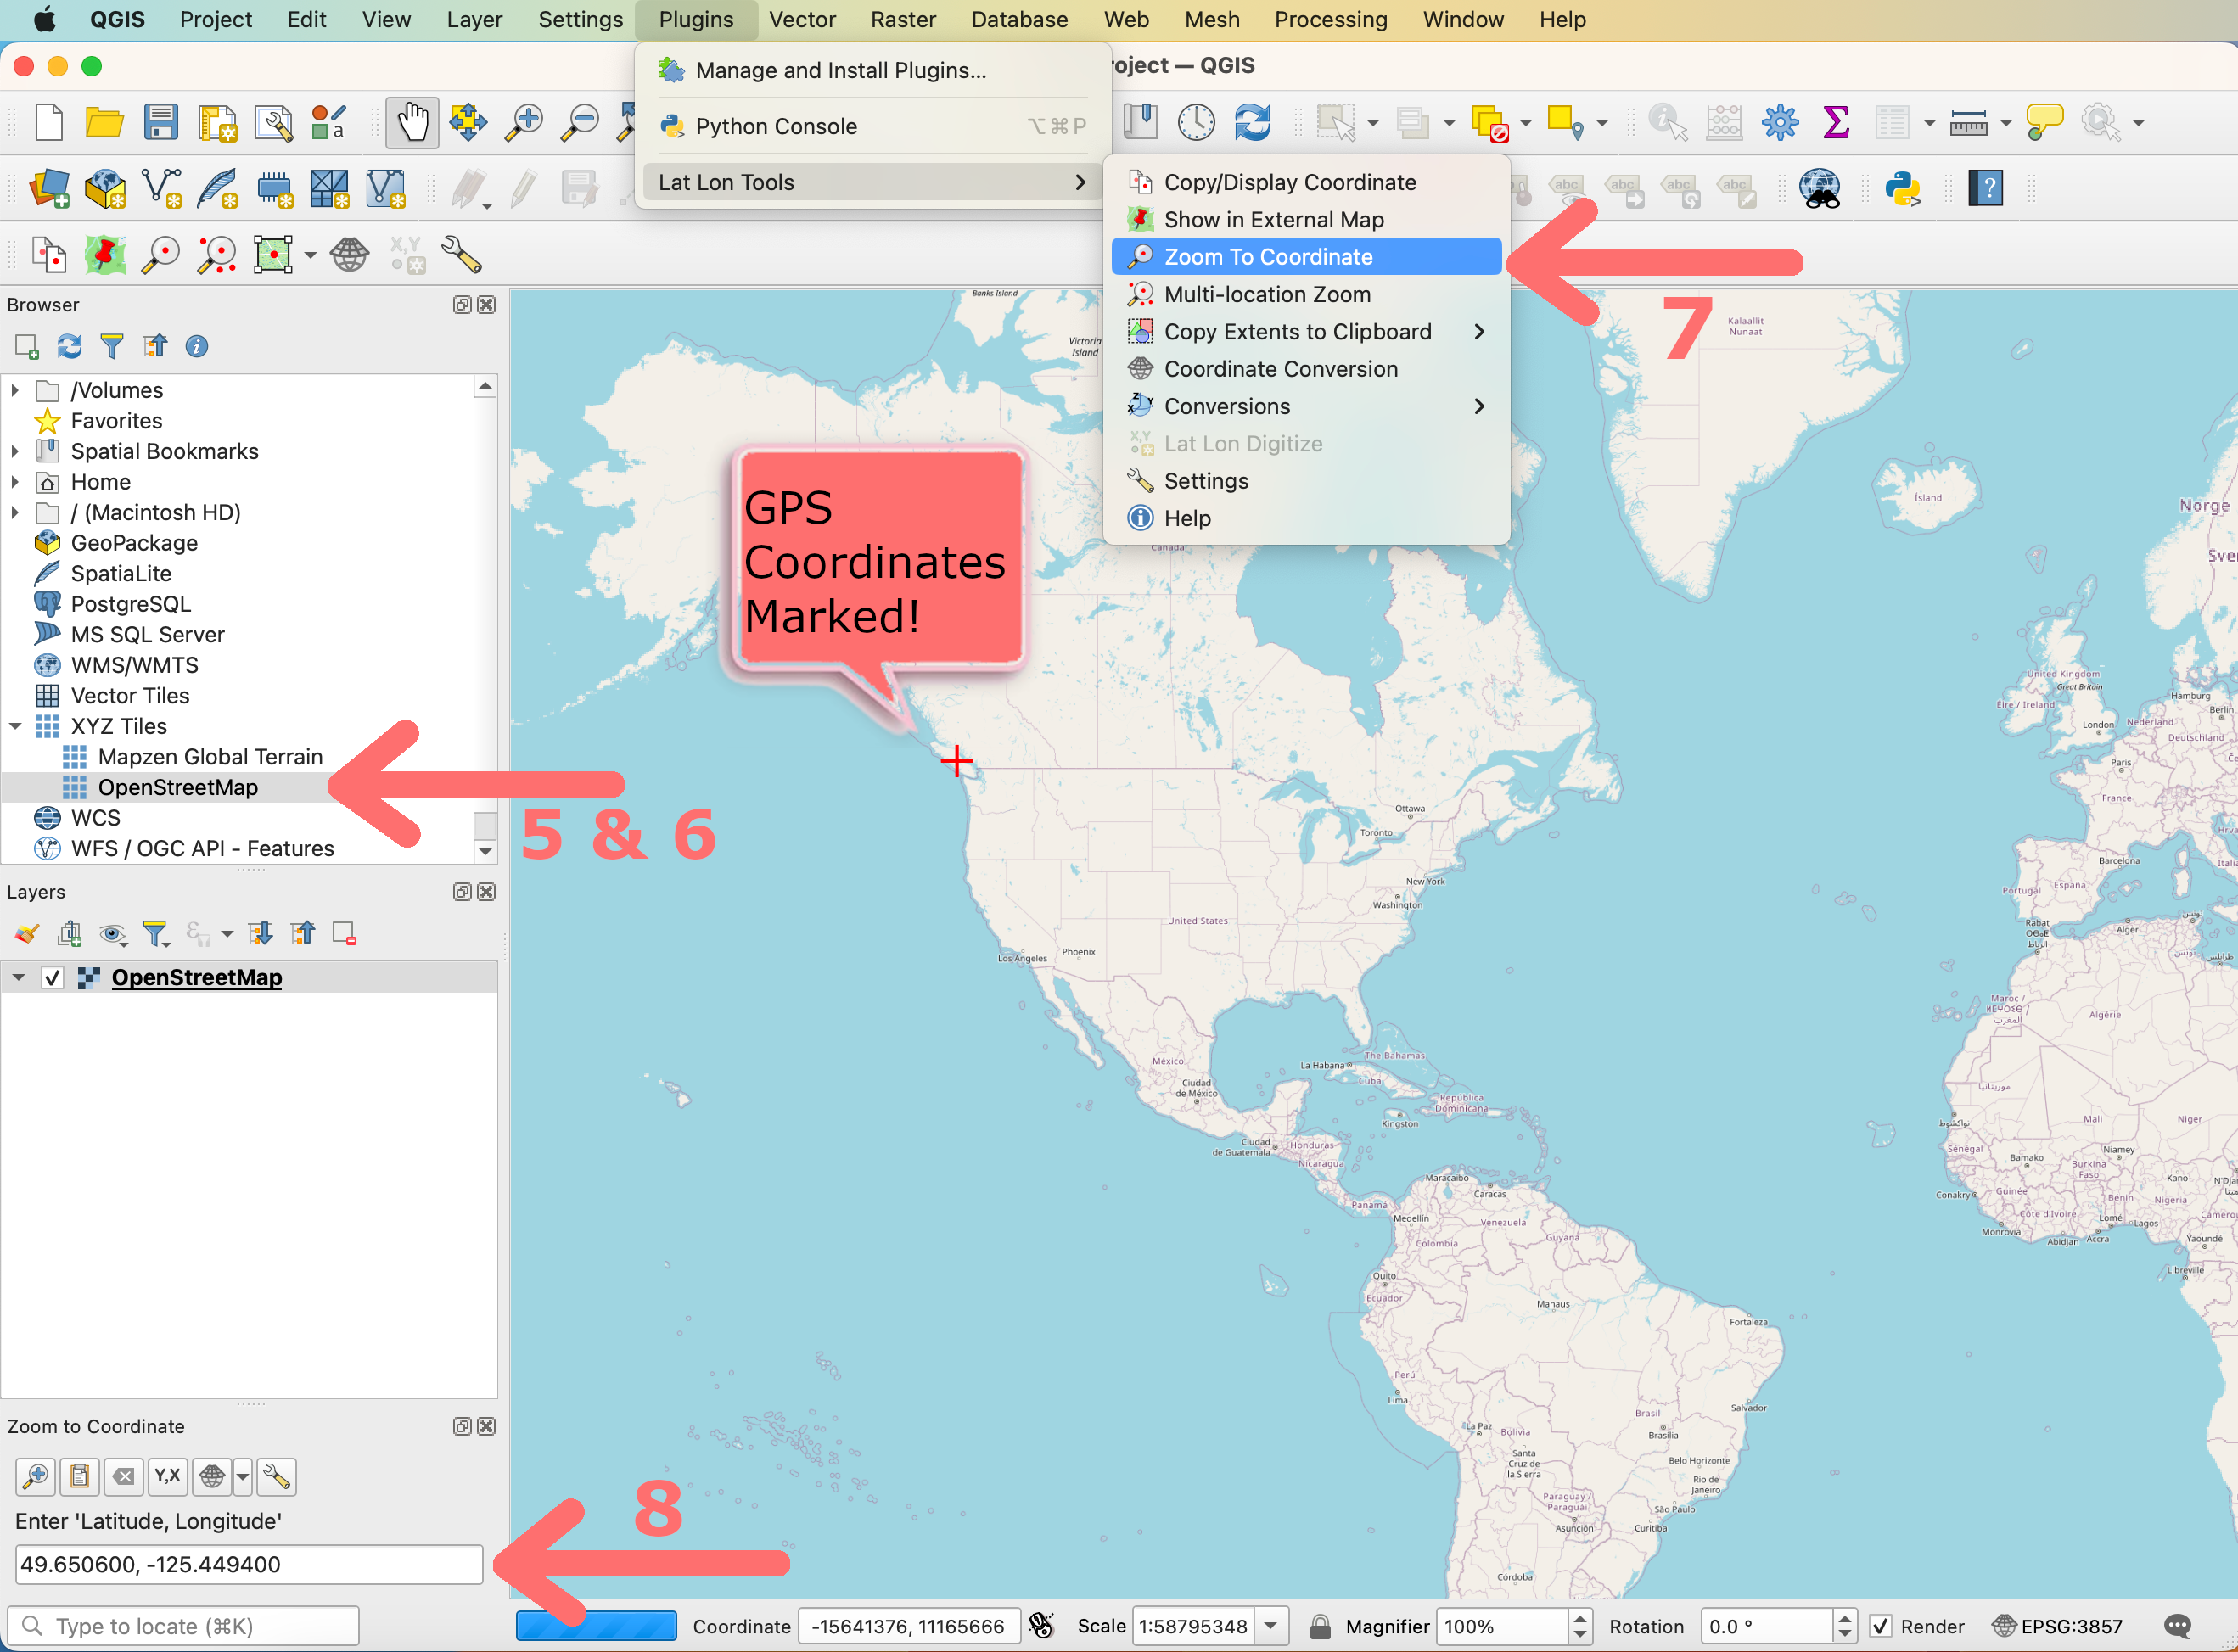
\includegraphics[width=.9\textwidth]{QGISbasemap.png}}
	
	5. In the browser window, expand your options by clicking on the small arrow next to \textit{XYZ Tiles}.
	
	6. Double click on Open Street Map to load in a basic open source map. You will notice that we just added a layer to the layer window below.
	
	\subsection{Finding GPS Coordinates with \textit{Lat Lon Tools}}
	
	Let's say you were interested in requesting and downloading ECOSTRESS land surface temperature (LST) data for Vancouver Island. You need to tell A$\rho\rho$EEARS where Vancouver Island is located, then request and download the data before you can make a map of the results. The first step is to find the island on the basemap we just added.
	
	7. Open up the Lat Lon Tools window by selecting the \textit{Plugins} menu $\rightarrow$ \textit{Lat Lon Tools} $\rightarrow$ \textit{Zoom To Coordinate}.
	
	8. Enter in the following GPS coordinates (formatted as latitude, longitude) : 49.650600, -125.449400. If you are not sure of the latitude and longitude of a location, you can navigate to that location in Google Maps and right-click on the location to display the coordinates. 
	
	9. The Lat Lon Tools plugin has found the GPS coordinates for Vancouver Island and marked them with a ``$+$'' on the map. 
	
	\subsection{Drawing a Shapefile}
	
	\centerline{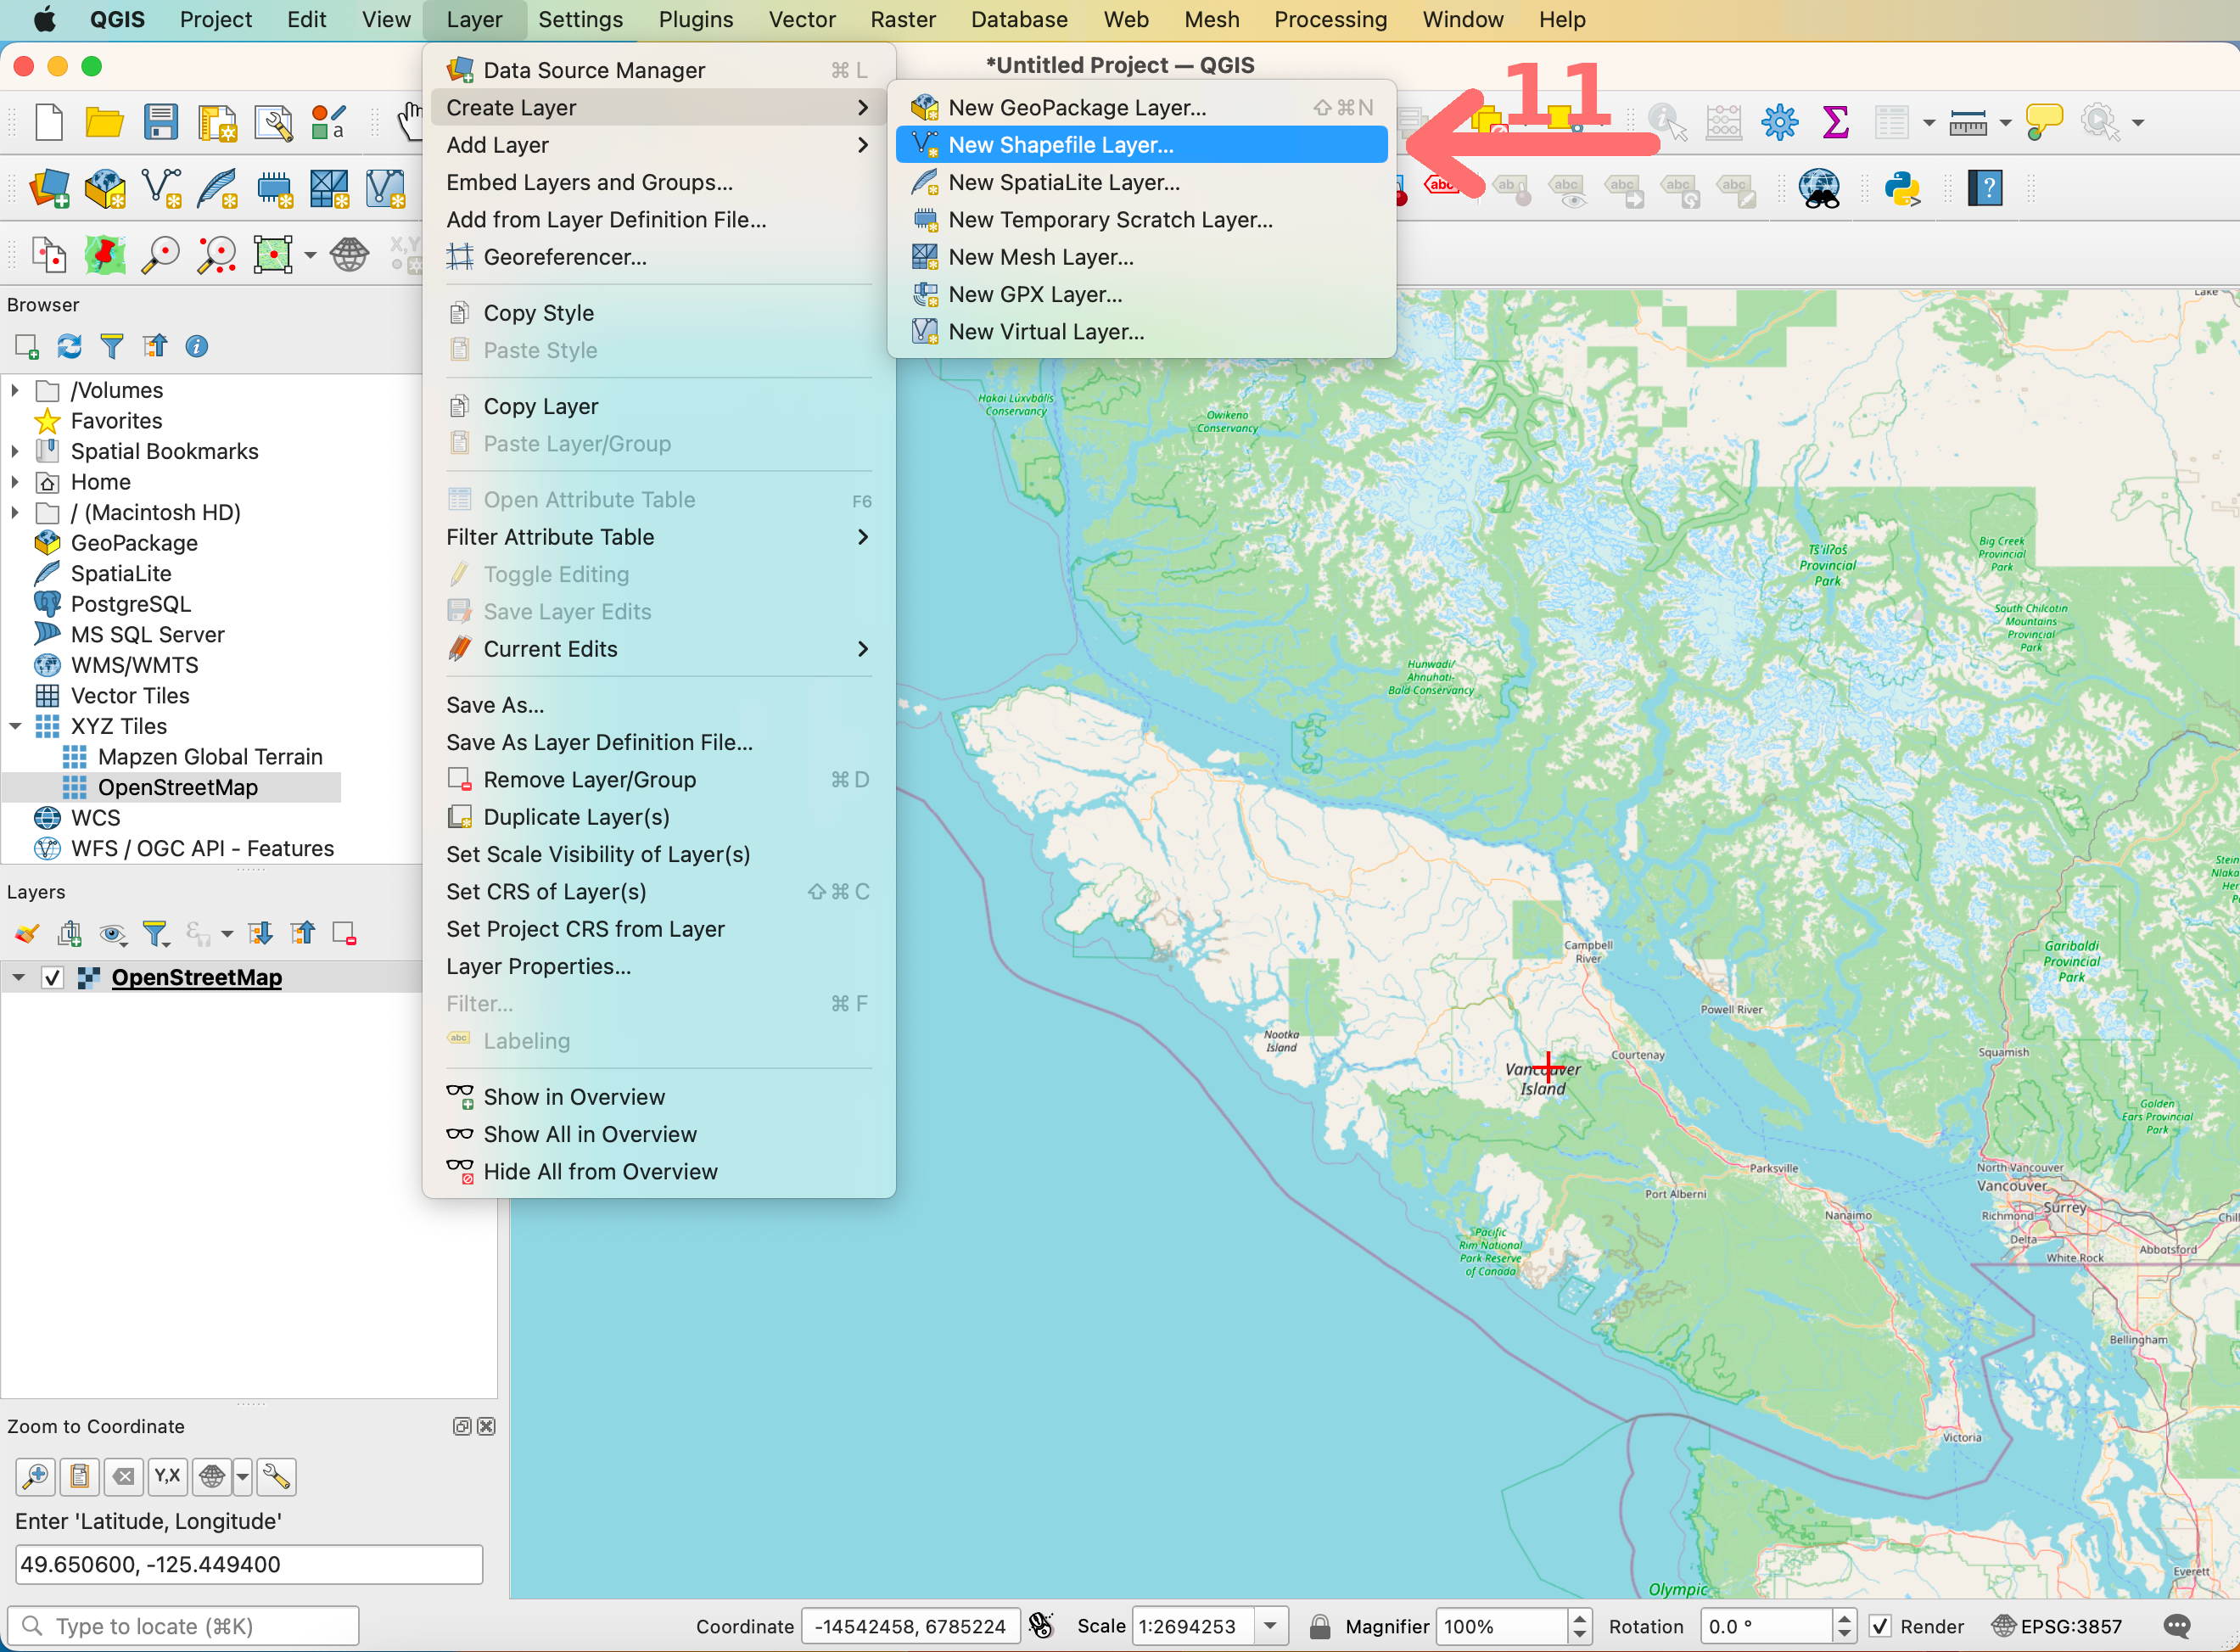
\includegraphics[width=.9\textwidth]{CreateLayer.png}}
	
	Next, we want to draw a polygon (i.e., a line that forms the perimeter of the area of interest) that encompasses Vancouver Island, so that we can request and download the data from A$\rho\rho$EEARS.
	
	10. Zoom in to the GPS coordinates that we entered and marked with a ``$+$'' on the basemap using the \textit{zoom in} 
\includegraphics[height=\fontcharht\font`\B]{mActionZoomIn.png}, \textit{zoom out} 
\includegraphics[height=\fontcharht\font`\B]{mActionZoomOut.png}, and \textit{pan} 
\includegraphics[height=\fontcharht\font`\B]{mActionPan.png} buttons in the toolbar. If you are on a laptop, you can use the trackpad to do the same.
	
	11. Next, we are going to create a new layer on the map by selecting the following menus: \textit{Layer} $\rightarrow$ \textit{Create Layer} $\rightarrow$ \textit{New Shapefile Layer...}
	
	\centerline{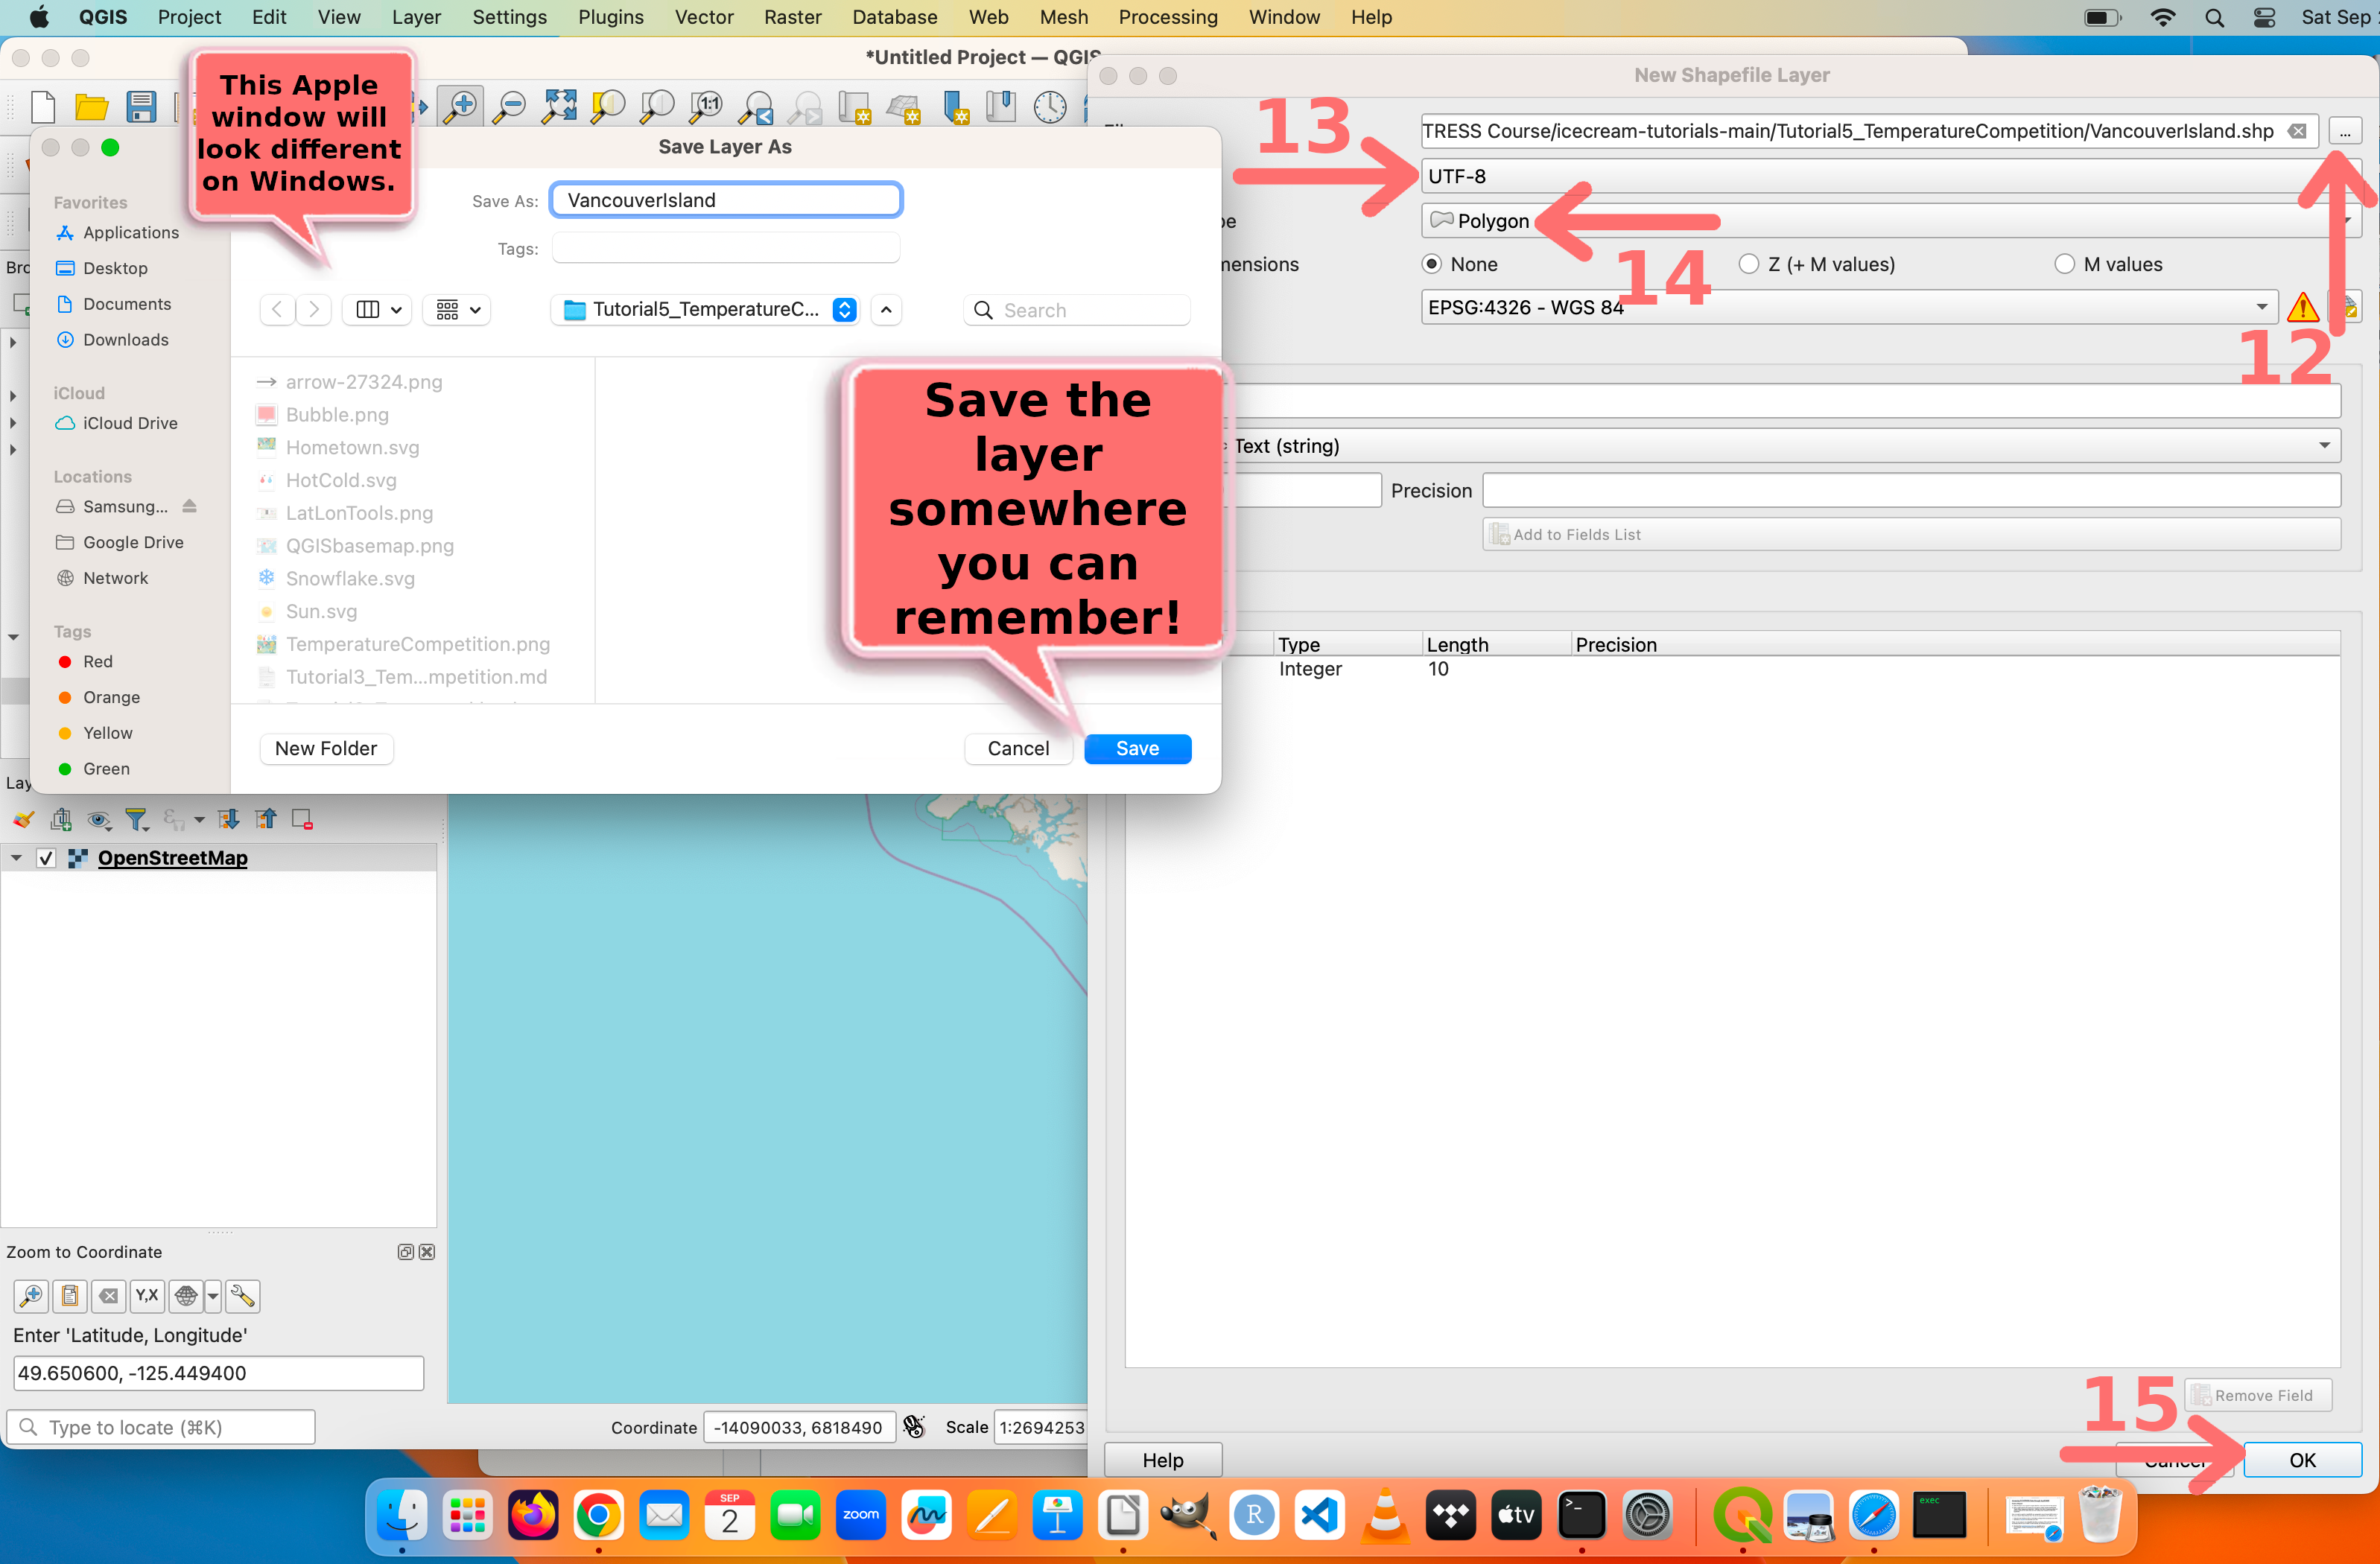
\includegraphics[width=.9\textwidth]{SaveLayer.png}}
	
	12. Select the ``...'' option next to the \textit{Filename} input window. Navigate somewhere you can remember and save it with an appropriate filename, such as ``Vancouver Island Perimeter."
	
	13. Select \textit{UTF-8} for \textit{File encoding}.
	
	14. Select \textit{Polygon} for geometry type. 
	
	15. Leave the remaining options as their defaults and click \textit{OK}.
	
	\centerline{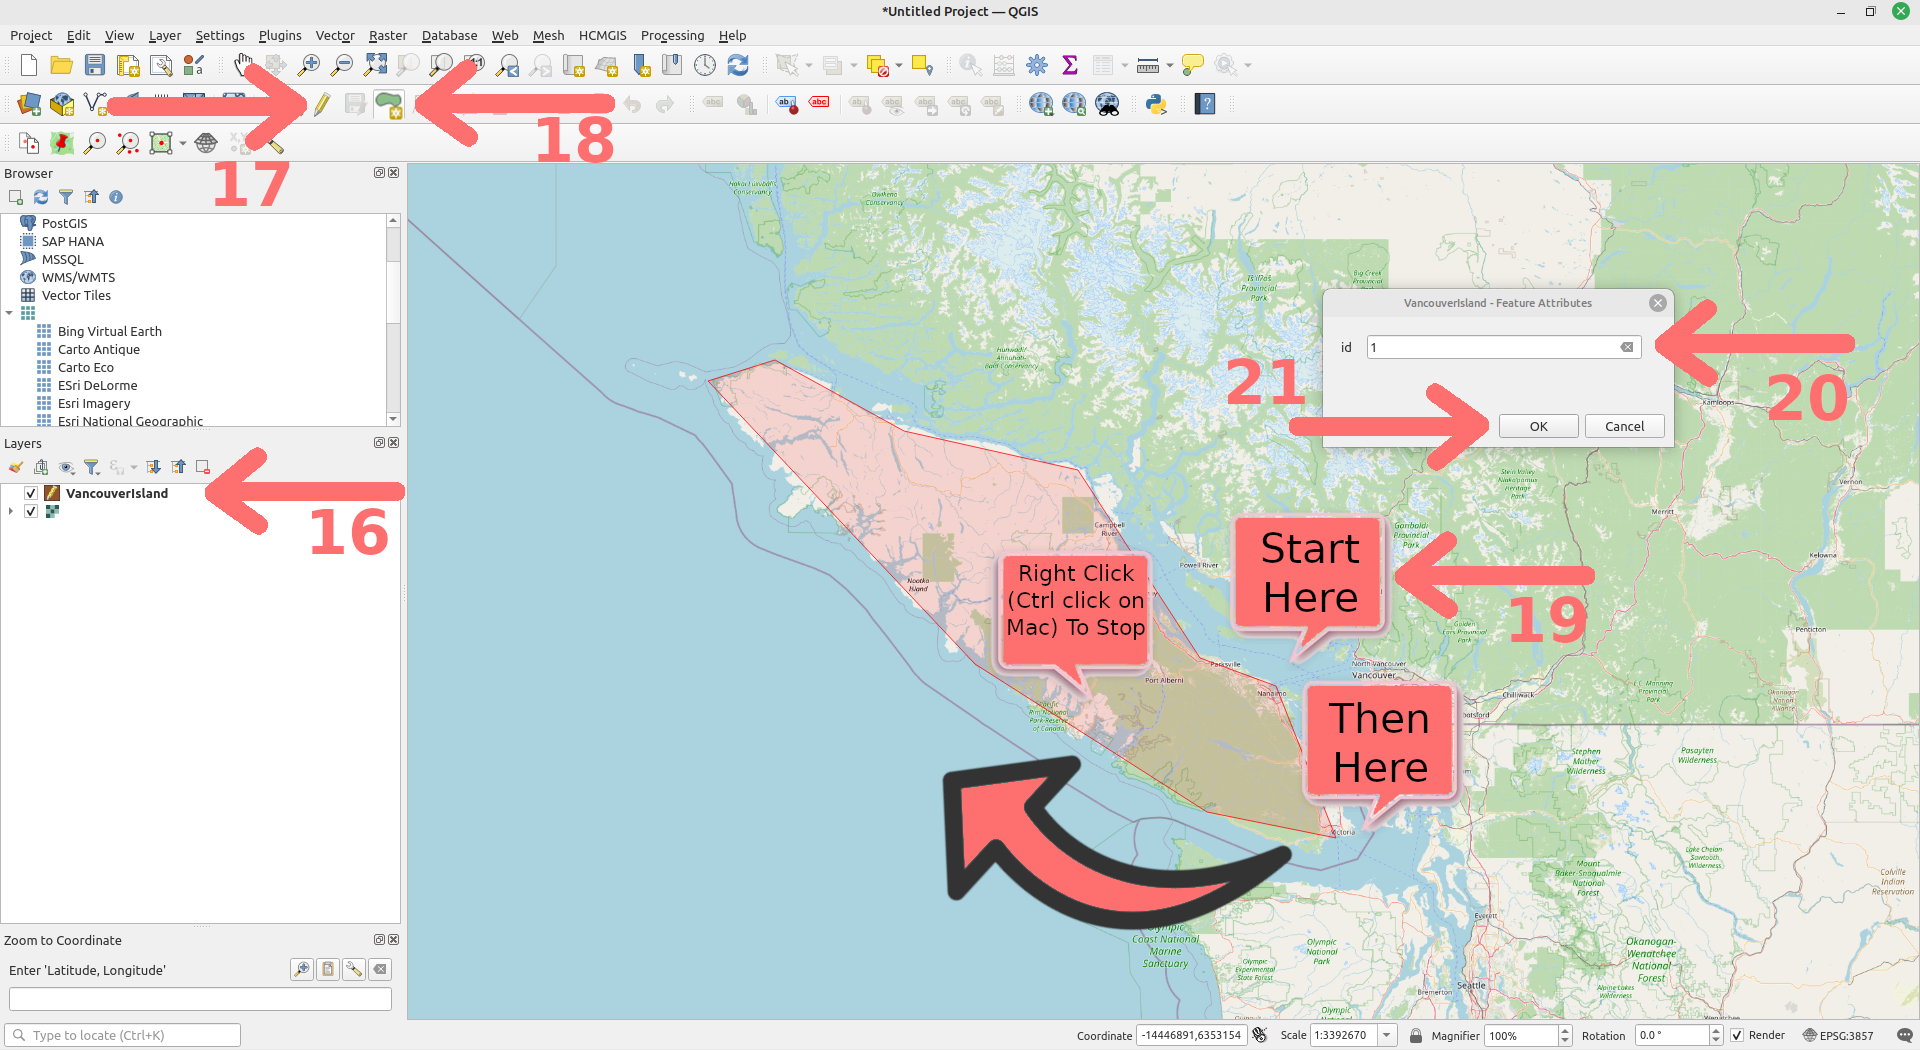
\includegraphics[width=\textwidth]{DrawPolygon.png}}
	
	16. Now, it is time to draw the polygon. First, make sure that your new ``Vancouver Island'' layer is highlighted in the \textit{Layers} window. 
	
	17. Select the \textit{Toggle Editing} 
\includegraphics[height=\fontcharht\font`\B]{mActionToggleEditing.png} button from the toolbar to start editing the layer. 
	
	18. Then select the \textit{Add Polygon Feature} 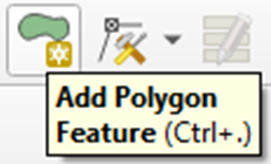
\includegraphics[height=10mm]{addpolygon.png} button to begin drawing your shapefile. 
	
	19. Draw a polygon that encompasses Vancouver Island. Don't worry too much about being perfect, getting the basic shape will do. Right-click on Windows or Linux and Ctrl-click on Mac to stop drawing when your shape is complete.
	
	\kulbox{\textbf{NOTE:} Drawing a polygon in QGIS is both straightforward and nuanced. You use successive clicks with your mouse to create your desired shape. Simple forms like squares or rectangles are easy achievable, while more complex designs take some practice to master. Our recommended route is to start by clicking near Parksville then proceed clockwise around the island. See the screenshot above (step 19).}
	
	20. After you finish drawing, QGIS will prompt you for a feature ID. This is an arbitrary designation for our purposes today, so simply using the number 1 is fine. 
	
	21. Click \textit{OK}. 
	
	22. Select the \textit{Toggle Editing} 
\includegraphics[height=\fontcharht\font`\B]{mActionToggleEditing.png} button from the toolbar to toggle off editing the layer. QGIS will prompt you to confirm saving the layer. Select \textit{Yes}. QGIS has now saved a shapefile with your polygon. 
	
	\begin{tcolorbox}[colback=yellow!5!white,colframe=IceCreamLeaf,title=\textbf{What Are Shapefiles?}]
		The shapefile format is one of the most commonly used vector file formats for geographic information. A shapefile dataset consists of several files. The following three are required:
			
		\begin{itemize}
			\centering
			\item[\color{orange} .shp] file containing the feature geometries
			\item[\color{orange} .dbf] file containing the attributes in \href{https://en.wikipedia.org/wiki/.dbf}{dBase} format
			\item[\color{orange} .shx] index file
		\end{itemize}
			
		Additionally, they can have: 
			
		\begin{itemize}
			\centering
			\item[\color{orange} .prj] which contains projection information
			\item[\color{orange} .cpg] plain text files that describes the encoding applied
			\item[\color{orange} .qix] spatial index file containing zoom and pan information
		\end{itemize}			
	\end{tcolorbox}
	
	23. The A$\rho\rho$EEARS interface we use to access ECOSTRESS data requires shapefiles to be combined in a single \href{https://en.wikipedia.org/wiki/ZIP_(file_format)}{zip file}. Use the following instructions on the next page for your operating system to 'zip' the shapefile data.
	
	\begin{tcolorbox}[colback=yellow!5!white,colframe=blue!60!green,title=\flushright{Windows \hspace{.25em} 
\includegraphics[width=1cm]{WindowsLogo.png}}]
		\begin{enumerate}
			\item Locate the Vancouver Island shapefile layer files that you saved in step 12 using your computer's \textit{File Explorer} application 
\includegraphics[width=1cm]{Windows_11_Explorer.png} .
			\item Hold the \textit{ctrl} button down and select the files with the .shp, .dbf, .shx, .prj, and .cpg extensions. 
			\item When they are all selected, release the \textit{ctrl} button and right-click the highlighted files, select \textit{Send to}, and then select \textit{Compressed (zipped) folder}.
			\item A new zipped file with the same name is created in the same location. To rename it right-click the .zip file, select \textit{Rename}, and then type the new name. ``VancouverIsland.zip'' seems like a good choice.
			\item This .zip shapefile dataset is now ready to be used in A$\rho\rho$EEARS.
		\end{enumerate}
	\end{tcolorbox}
	
	\begin{tcolorbox}[colback=yellow!5!white,colframe=red!70!white,title=\flushright{Apple macOS \hspace{.25em} 
\includegraphics[width=1cm]{AppleLogo.png}}]
		\begin{enumerate}
			\item Locate the Vancouver Island shapefile layer files that you saved in step 12 using your computer's \textit{Finder} application 
\includegraphics[width=1cm]{Finder.png} .
			\item Hold the \textit{command} button down and select the files with the .shp, .dbf, .shx, .prj, and .cpg extensions. 
			\item When they are all selected, release the \textit{command} button and ctrl-click the highlighted files, select \textit{Compress}, and then select \textit{Compressed (zipped) folder}.
			\item A new zipped folder with the name ``Archive.zip'' is created in the same location. To rename it, ctrl-click the folder, select \textit{Rename}, and then type the new name. ``VancouverIsland.zip'' seems like a good choice.
			\item This .zip shapefile dataset is now ready to be used in A$\rho\rho$EEARS.
		\end{enumerate}
	\end{tcolorbox}
	
In a future tutorial, we will use this shapefile to make an A$\rho\rho$EEARS request and download ECOSTRESS data, so remember the folder where you save it. 

	%%%%%%%%%%%%%%%%%%%%%%%%%%%%%%%%%%%%%%%%%%%%%%%%%%%%%%%%%%%%%%%%%%%%%%%%%%%%%%%%%%% Begin End Matter
	
	\vspace{.25em}
	
	\hrule
	
	\vspace{1 em}
	
	\begin{tcolorbox}[colback=yellow!5!white,colframe=IceCreamOrbit,title= \vspace{.2em} \Large Map of the Week Assignments]
		\addcontentsline{toc}{section}{Map of the Week Assignments}
		\large
            Over the next several tutorials you will learn the skills necessary to enter a contest to see who has the hottest/coldest hometown or favorite place you have lived. For today, let's focus on the first step of drawing a polygon around your hometown:
		\begin{enumerate}
			\item  Submit a map of your hometown (however you choose to define it), complete with the boundary of your shapefile outlined in the color of your choice. You may want to refer to \href{https://jeremydforsythe.github.io/icecream-tutorials/Tutorial2_MakingBasicMapsInQGIS/Tutorial2_MakingBasicMapsInQGIS.pdf}{Tutorial \#2 : Making Basic Maps in QGIS} for reference, since this is a similar process to the timezone map. When you think about your hometown, you need to consider scale. Will you draw a polygon around your house, your neighborhood, or the town/city as a whole? Down the road, this will affect how much data you end up visualizing. 
		\end{enumerate}
	\end{tcolorbox}
	
	\vfill
	
	\hrule
	
	\vspace{1em}
	
	\textbf{Recommended Citation:} Forsythe, J.D., G.R. Goldsmith, and J.B. Fisher. 2023. Observing Earth from Above Tutorials. Chapman University. \url{https://jeremydforsythe.github.io/icecream-tutorials/}
	
	\vspace{1em}
	
	This work is supported by funding from NASA ECOSTRESS Mission Grant \#80NSSC23K0309 (I.C.E. C.R.E.A.M.: Integrating Communication of ECOSTRESS Into Community Research, Education, Applications, and Media) and is openly licensed via \href{https://creativecommons.org/licenses/by-nc/4.0/}{CC BY-NC}.
	
\end{document}
